\documentclass[border=3pt,tikz]{standalone}
\usepackage{amsmath}
\usetikzlibrary{calc}
\usetikzlibrary{arrows.meta} % for arrow size
\begin{document}
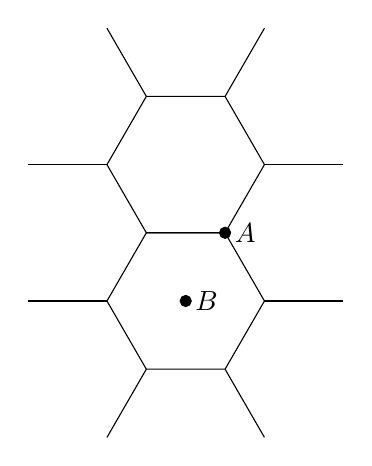
\begin{tikzpicture}

    \coordinate (A1) at (1, 0);
    \coordinate (A2) at ({cos(60)}, {sin(60)});
    \coordinate (A3) at ({cos(120)}, {sin(120)});
    \coordinate (A4) at ({cos(180)}, {sin(180)});
    \coordinate (A5) at ({cos(240)}, {sin(240)});
    \coordinate (A6) at ({cos(300)}, {sin(300)});

    \draw[] (A1) -- (A2) -- (A3) -- (A4) -- (A5) -- (A6) -- cycle;
    \draw[] ($(A1) + (0, {2*sin{60}})$) -- ($(A2) + (0, {2*sin{60}})$) -- ($(A3) + (0, {2*sin{60}})$) -- ($(A4) + (0, {2*sin{60}})$) -- ($(A5) + (0, {2*sin{60}})$)-- ($(A6) + (0, {2*sin{60}})$) -- cycle;
    \draw[] ($(A2) + (0, {2*sin{60}})$) -- ($(A2) + ({cos(60)}, {3*sin{60}})$);
    \draw[] ($(A3) + (0, {2*sin{60}})$) -- ($(A3) + ({-cos(60)}, {3*sin{60}})$);
    \draw[] ($(A4) + (0, {2*sin{60}})$) -- ($(A4) + (-1, {2*sin{60}})$);
    \draw[] ($(A4) + (0, 0)$) -- ($(A4) + (-1, 0)$);
    \draw[] ($(A5) + (0, 0)$) -- ($(A5) + ({-cos(60)}, {-sin{60}})$);
    \draw[] ($(A6) + (0, 0)$) -- ($(A6) + ({cos(60)}, {-sin{60}})$);
    \draw[] ($(A1) + (0, 0)$) -- ($(A1) + ({1}, {0})$);
    \draw[] ($(A1) + (0, {2*sin{60}})$) -- ($(A1) + ({1}, {2*sin{60}})$);
    
    \filldraw[black] (0,0) circle (2pt) node[right] {$B$};
    \filldraw[black] (A2) circle (2pt) node[right] {$A$};
    
\end{tikzpicture}
\end{document}